\section{Projektinitialisierung}\label{sec:Projektinitialisierung}

Der Rahmen des Projekts... 

\subsection{Unternehmen}

Wir sind ein junges Unternehmen bestehend aus drei Studenten der Sozialinformatik. Wir setzen uns zusammen aus zwei Softwareentwicklern (Backend- und Frontendentwickler) und einem Netzwerkadministrator. Das unternehmen wurde im Jahr 2018 im Zuge eines IT-Projekts für unser Studium gegründet.


\subsection{Projekt}

\textit{Was ist das für ein Projekt? Was soll es bringen? }

Die freiwillige Feuerwehr von Eschenstruth gibt Feuerwehrkleidung für anliegende Ortsteile an Kinder aus. Dies gestaltet sich zunehmend schwerer, da die aktuelle Bestandspflege und der Überblick über die ausgegebene Kleidung mit den aktuellen Methoden schwer fällt. Vor wenigen Jahren wurden die Ausgabe und Verwaltung der Kleidung noch mit Zetteln dokumentiert. Dabei kam es durch uneinheitliches Vorgehen zu Verlust von Informationen. Dies geschah \zb durch den Verlust eines Zettels. Ein Zettel konnte schnell geschrieben, musste aber auch ordentlich in die entsprechende Akte eingepflegt werden. Zudem musste der Ort der Akte erst aufgesucht werden um das Schriftstück ab zuheften. 
Aktuell wird eine Excel"=Tabelle gepflegt. Diese befindet sich auf einem lokalen Rechner und einem USB"=Stick zur Datensicherung. Hier besteht der Nachteil, dass ein Rechner, auf dem sich de Excel"=Tabelle befindet, aufgesucht werden muss, um den Kleidereingang oder "=ausgang aus dem Lager zu dokumentieren. Als Zwischenspeicher wird eine Tafel verwendet, die bei der Ausgabe oder Annahme von Kleidung gefüllt wird (s. Abbildung~\ref{fig:tafel}). Der Warenbestand kann dann von einem beliebigen Rechner aus übertragen und dokumentiert werden, unter der Voraussetzung, dass die Person die aktuelle Excel"=Tabelle besitzt. Es muss aber bei der Synchronisation der Dokumentation darauf geachtet werden, dass die Daten in chronologisch richtiger Reihenfolge aufbereitet werden. Das kann unter Umständen, wenn zwei Personen zur gleichen Zeit an der Tabelle gearbeitet haben, zu einem erheblichen Mehraufwand führen, wenn nicht direkt nachvollziehbar ist, wer als letztes die Tabelle gepflegt hat, oder auf welchen Stand sich die Excel"=Tabelle befindet. 

\begin{figure}[hbtp]
  \centering
  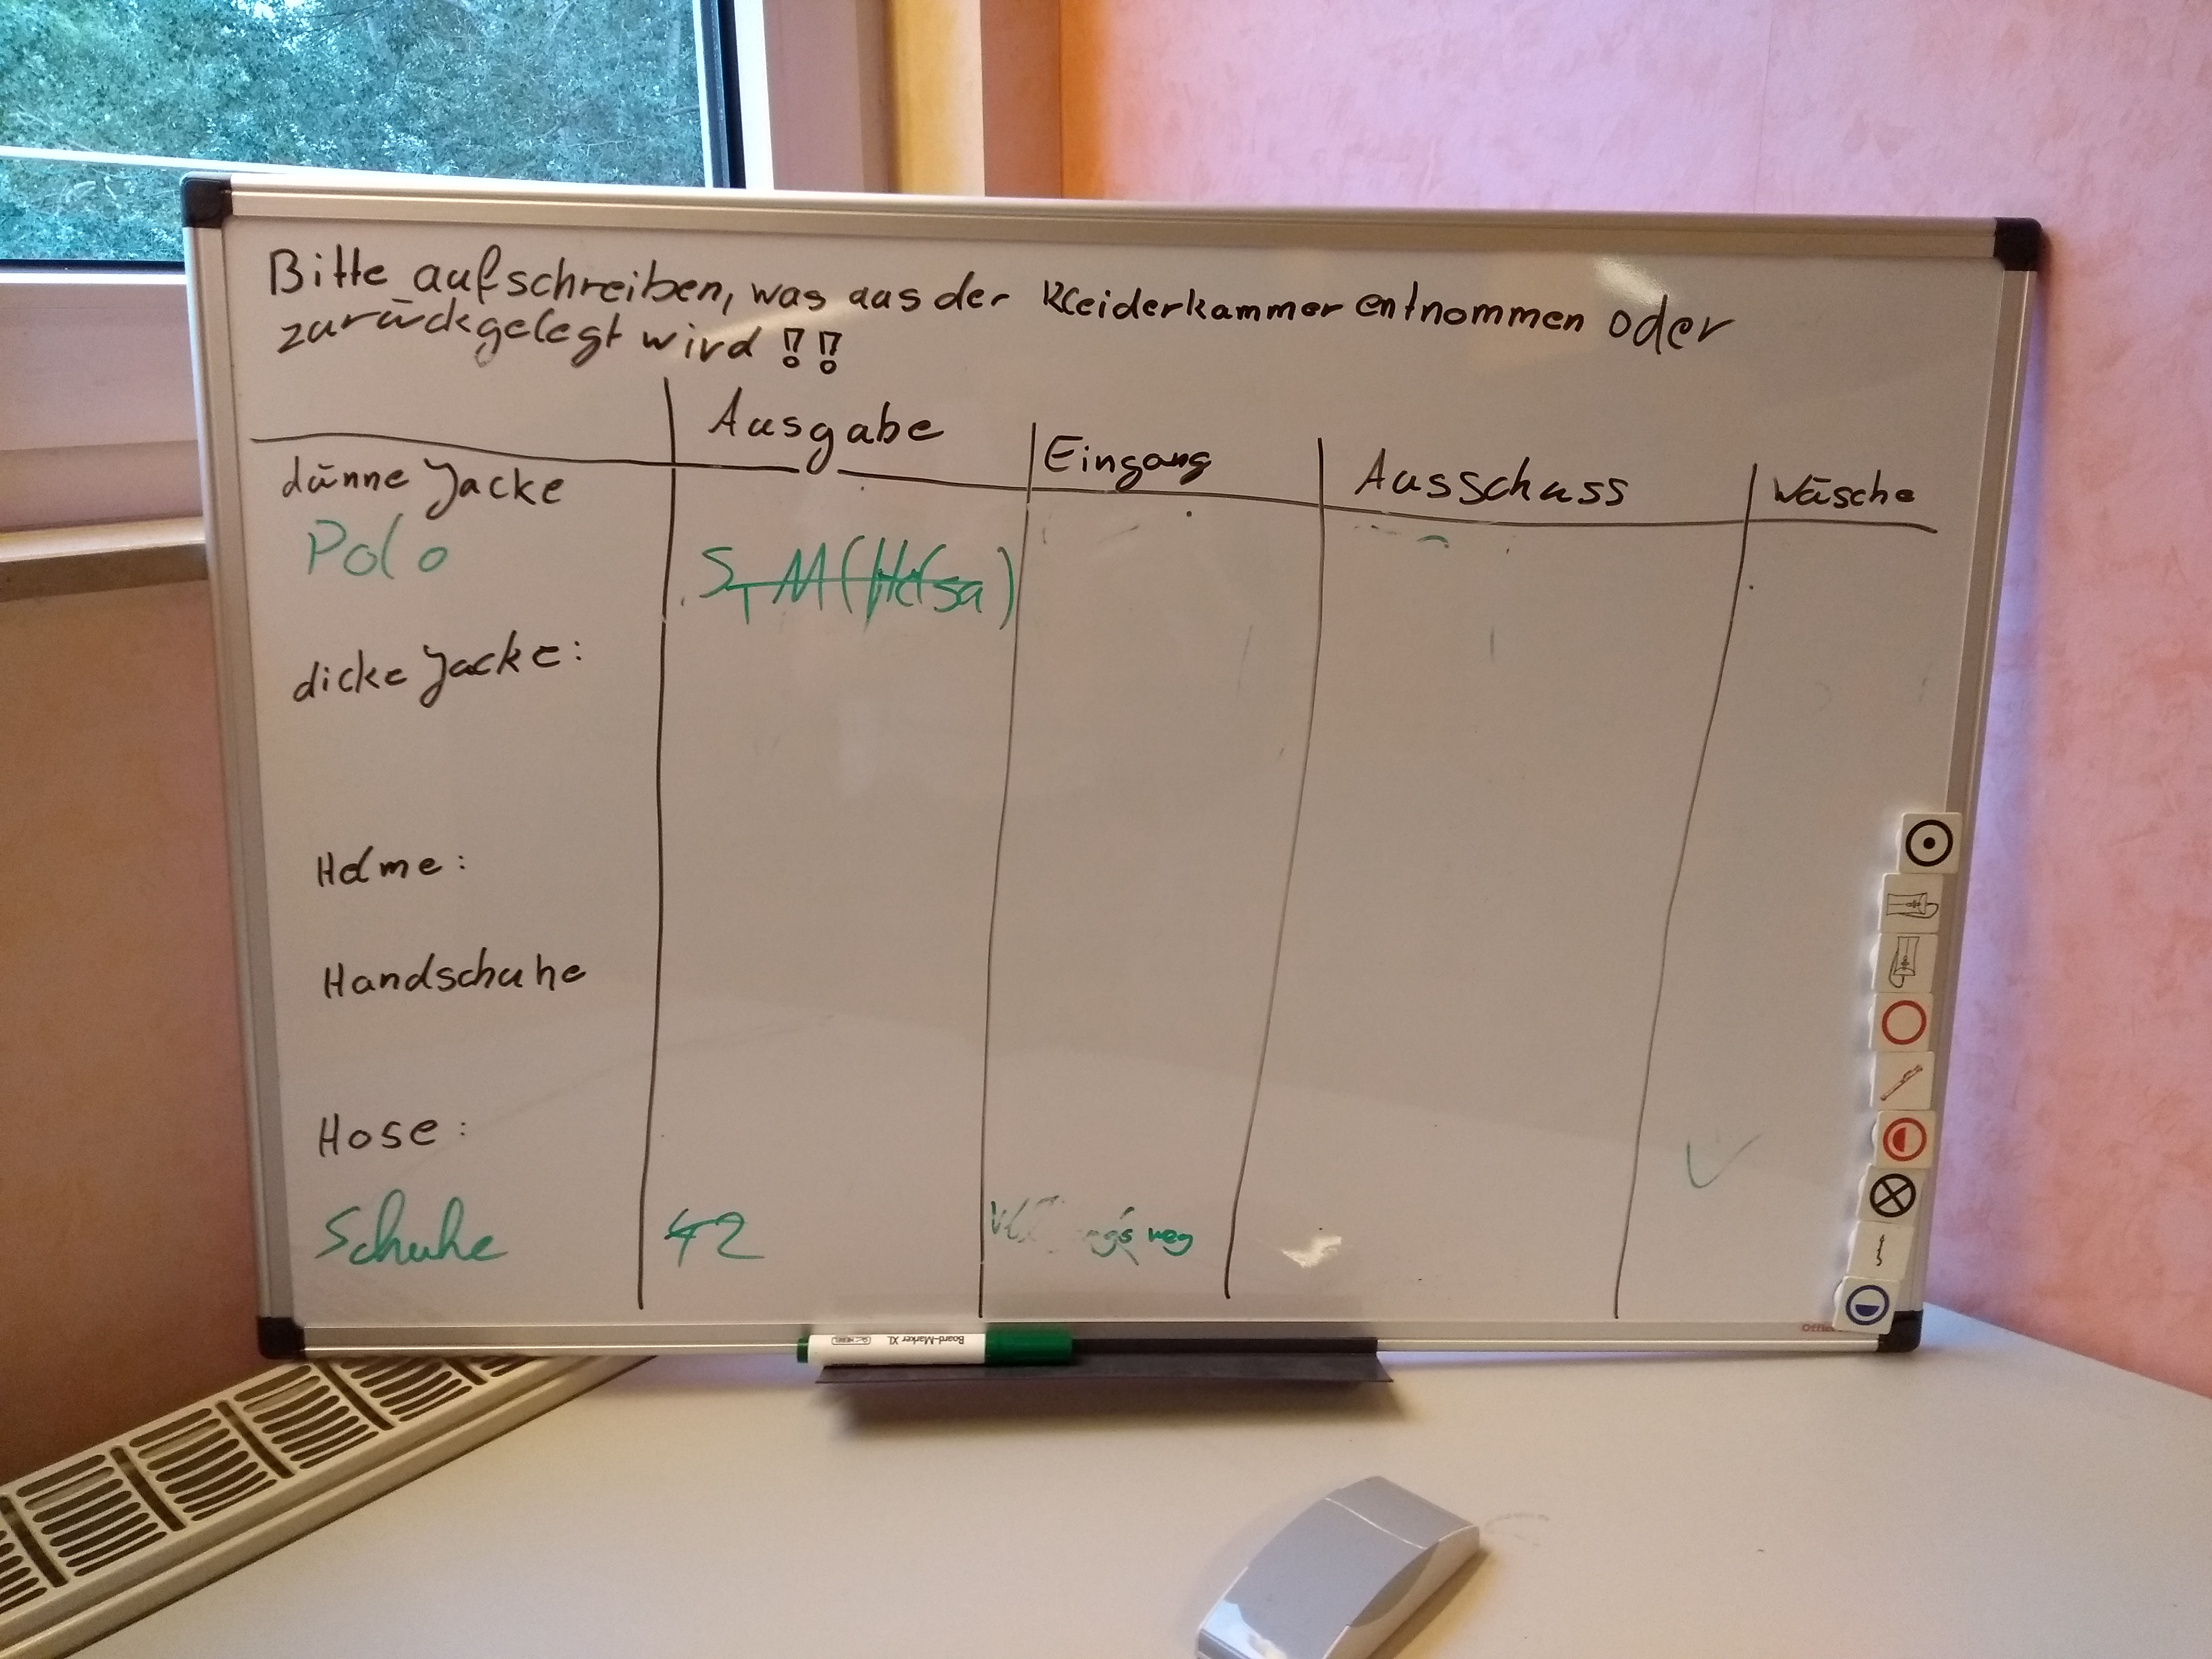
\includegraphics[width=0.95\textwidth]{res/IMG_20180815_193814370}
  \caption{Tafel aus Zwischenspeicher von Informationen.}
  \label{fig:tafel}
\end{figure}

Um die Probleme des Datenverlusts und der Synchronisation von Daten zu beseitigen, kam die Idee einer zentralen, aus dem Internet erreichbaren Kleiderverwaltung der Jugendfeuerwehr von Eschenstruth, oder auch \project, auf.

In den folgenden Kapiteln werden die Kernziele dieses Projekts erläutert und die Erfolgskriterien definiert. Die beteiligten Personen an diesen Projekt werden erfasst und kurz vorgestellt. Darauf folgt der Projektansatz mit der Anforderungsspezifikation. Dabei werden alle Anforderungen die zwingend in diesem Projekt umgesetzt werden müssen definiert. 

\subsection{Project Definition Document}

\subsubsection{Gegenstand, Kernziele und Ziele des Projektes}

\textit{Welches Ziel wird damit verfolgt?}

Ziel ist es eine vollständig nachvollziehbare Dokumentation zu ermöglichen, bei dem zu jederzeit der aktuelle Aufenthaltsort der zur Verfügung stehenden Kleidung ermittelt werden kann. Dabei soll ein paralleles Arbeiten möglich sein. Die Anwendung muss auch von mobilen Geräten bedienbar sein, damit nicht nur ein Computer verwendet werden muss. Sie muss zudem intuitiv bedienbar sein. 

\subsubsection{Erfolgskriterien}

\textit{An was werden die Erfolgskriterien festgelegt?}

Ein Erfolgskriterium ist die vollständige Ablösung der Excel"=Tabelle und der Tafel. Die Daten werden nur noch über die Anwendung gepflegt.

\textit{Fällt uns nochwas ein? Bitte melden!!}


\subsubsection{Kontext des Projektes und die Projektabhängigkeiten}

\textit{In welchem Rahmen findet das Projekt statt?}

Das Projekt findet im Kontext des Studiengangs Sozialinformatik (B.Sc.) der Hochschule Fulda statt.

\subsubsection{Risiken, die den Projekterfolg verhindern könnten}

\textit{Was für Risiken können im Verlauf des Projekts auftreten?}

Dadurch, dass das Projekt"=Team Vollzeit tätig ist, kann es zu Engpässen in der Durchführung kommen. Dies kann unter Umständen zu Mehrarbeit auf einzelne Team"=Mitglieder führen. Das Risiko ist gering einzuschätzen, da das Projekt"=Team  hinter der Idee steht.

Ein weiteres Risiko betrifft die Evaluation einer kostenlosen, bis kostengünstigen, Plattform, auf der die Anwendung bereit gestellt werden kann. Dabei kann die Akzeptanz der Endkunden sinken, wenn die Betriebskosten zu hoch ausfallen. Ab welchen Betrag die Kosten zu hoch sind, ist noch zu klären. Dieses Risiko ist mittelmäßig einzuschätzen, da es am Markt diverse Anbieter gibt. Unter den bekannteren Anbietern gehören \textit{AWS}, von \textit{Amazon}, und \textit{Heroku}.

\subsubsection{Am Projekt Beteiligte}\label{sec:beteiligte}

Zum Projekt"=Team gehören:

\begin{itemize}
\item Tim Wieder, ist zuständig für den Kundenkontakt und die Frontend"=Entwicklung.
\item Achim Rose, ist zuständig für die Backend"=Entwicklung und den Entwurf der Datenbanktabellen. 
\item Sebastian Seeger, ist zuständig für die Infrastruktur. Das betrifft die Evaluation der Plattform und dessen Konfiguration.
\end{itemize}

Zu den Kunden, sprich die Beteiligten der freiwilligen Feuerwehr Eschenstruth, gehören: 

\begin{itemize}
\item Nico M. (zuständig für die Kleiderkammer)
\item Julia W.
\item Marcel B.
\item Markus N.
\item Florian B.
\item Philipp H.
\end{itemize}

\subsubsection{Zu erwartender Projektansatz}

\textit{Wie wird das Projekt umgesetzt. Beschreibung der Vorgehensweise (agil und so)}

\section{Projektplanung}\label{sec:Projektplanung}

Diese Anforderungsspezifikation ist die Aufnahme der Bedürfnisse nach dem ersten Meeting mit den Stakeholdern. Durch die Verwendung von Scrum können wir durch die grobe Beschreibung der Anforderungen unsere Sprints planen und bei der Erstellung der Datenbankstruktur auf die Anforderungen zurück greifen. 


\subsection{Anforderungsspezifikation}

Die Anwendung wird in vier Abschnitte gegliedert: Startseite, Aktionen, Auswertungen und Administration.

Auf der \textit{\textbf{Startseite}} müssen die letzten 20 Transaktionen aufgelistet werden. Dabei werden die Informationen über die Transaktion selbst angezeigt, sowie die Person die die Transaktion ausgeführt hat.

Die Transaktionen, oder auch Aktionen, werden im Abschnitt \textit{\textbf{Aktionen}} durchgeführt. Eine Transaktion umschließt die Informationen der \textit{Kleidungsart}, \textit{Stückzahl}, \textit{Größe}, \textit{Bestimmungsort}, \textit{Art der Aktion} und der \textit{ausführenden Person}. Bei einer Transaktion müssen immer die Informationen über die Kleidungsart, die Stückzahl, die Größe und den Bestimmungsort angegeben werden. Dabei werden Kleidungsart, Größe und Stückzahl in einer Gruppe erfasst damit mehrere Kleidungsarten in einer Transaktion an einen Bestimmungsort übergeben werden können. 

Über die Art der Aktion können der Anwender*innen festgelegen, ob die Kleidungsstücke an einen Bestimmungsort \textit{ausgegeben}, \textit{zurückgenommen} oder \textit{ausgesondert} werden. Kleidungsstücke können auch in die Wäsche gegeben werden. Dies ist notwendig um den Überblick über den Bestand zu wahren und nicht bei Mangel während der Ausgabe die Notwendigkeit zu sehen, Kleidungsstücke zu bestellen.

Der \textit{Bestimmungsort} kann ein Ortsteil der Feuerwehr sein oder das Lager, \bzw der Wareneingang. Somit lässt sich erkennen, ob Kleidungsstücke in den Warenbestand aufgenommen wurden, oder an einen Ortsteil ausgegeben wurde.
Aus den Aktionen resultiert für die Startseite die Liste der Transaktion in natürlich sprachlichen Texten. Zum Beispiel: 
\begin{itemize}
\item 5 dünne Jacken in Größe 40 vom Ortsteil Helsa ausgesondert, durch Max Mustermann am 14.12.2019 09:43 Uhr.
\item 12 Hosen in Größe 32 ins Lager aufgenommen, durch Max Mustermann am 10.12.2019 15:26 Uhr.
\item 12 Hosen in Größe 32 vom Lager in der Wäsche, durch Max Mustermann am 10.12.2019 12:02 Uhr.
\item 10 Jacken in Größe 40, 10 Stiefel in Größe 36 vom Ortsteil Helsa ausgegeben, durch Max Mustermann am 06.12.2019 18:12 Uhr.
\item 10 Jacken in Größe 40, 10 Stiefel in Größe 36 vom Wareneingang aufgenommen, durch Max Mustermann am 05.12.2019 17:30 Uhr.
\end{itemize}

Die Kleidungsstücke und deren Größen, sowie die Ortsteile und die Anwender*innen, können in der \textbf{\textit{Administration}} verwaltet werden.

In der Administration der Ortsteile können beliebige Ortsteile nach Bedarf hinzugefügt werden. Dabei muss der Name angegeben werden und ein Ansprechpartner. Optional können weitere Ansprechpartner zu einem Ortsteil hinzufügt oder bis auf einen entfernt werden. Ein Ortsteil kann auch inaktiv gesetzt werden. Hierbei muss jedoch geprüft werden, ob sich noch Kleidungsstücke auf den Ortsteil gebucht sind. Das Inaktiv setzen ist erst dann möglich, wenn alle Kleidungsstücke in den Warenbestand zurück gebucht wurden. Es bietet sich an, dafür eine Komfort"=Funktion bereit zu stellen. Diese Transaktion muss auch über die Startseite erkennbar sein. Ein Ortsteil kann deshalb nicht gelöscht werden, weil durch den Verlust der Information die Transaktionen nicht mehr vollständig nachvollziehbar wären. Ein Ortsteil kann nur dann effektiv gelöscht werden, wenn keinerlei Transaktionen darauf ausgeführt wurden.

Am Ortsteil können Grenzen der Anzahl von Kleidungsstücken bestimmt werden, bei dem eine Warnung erscheint, wenn zu viele Kleidungsstücke ausgegeben wurden. Diese Warnung erscheint bei den Aktionen nach der Auswahl des Ortsteils. Wenn keine Grenze angegeben wurde, wird nichts geprüft.

Ein weiterer Punkt der Administration ist die Benutzerverwaltung. Hier können Personen angelegt und gelöscht, ihre Rechte verwaltet und der Einkäufer bestimmt werden. Dazu müssen der Name, die E"=Mail Adresse gespeichert werden. Zudem kann gesteuert werden, ob die Person nur lesenden, schreibenden oder administrativen Zugriff auf das System hat. Bei lesendem Zugriff ist die Seite der Aktionen gesperrt. Bei schreibenden Zugriff ist die Seite der Administration gesperrt. Der Administrator hat auf alle Bereiche Zugriff. Die Einstellung, ob eine Person für den Einkauf zuständig ist, ist mit der Administration der Kleidungsstücke verknüpft. 

Die Kleidungsarten und die dazugehörigen Größen können in der Administration erweitert werden. Diese können nur gelöscht werden, wenn noch keine Transaktionen mit der Kleidungsart und Größe vorgenommen wurde. Dies ist besonders wichtig, damit die Auswertungen auch weiterhin nachvollziehbar und reproduzierbar sind. Kleidungsarten können aber inaktiv gesetzt werden, wodurch diese bei Aktionen nicht mehr ausgewählt werden können. Zu jeder Kombination von Kleidungsart und Größe kann ein Grenzwert festgelegt werden, bei dem die Einkäufer*innen eine E"=Mail Benachrichtigung erhalten. Damit diese Grenze nicht bei jeder Neuanlage eingetippt werden muss, kann der Standardwert angegeben werden.

Im Abschnitt der \textit{\textbf{Auswertungen}} können die Anwender*innen eine Bericht erstellen, der Auskunft über die ausgegebenen, zurückgenommenen und ausgesonderten Kleidungsstücke gibt. Dabei kann in einem Filter der Zeitraum, die Kleidungsart, Größe, Transaktionsart, der Ortsteil (wie auch der lokale Warenbestand) gesetzt werden, wodurch der Bericht auf spezielle Bedürfnisse angepasst werden kann. Der Bericht soll als Excel"=Tabelle oder PDF erfolgen.

\subsection{Projektplan}
\subsubsection{Work-Breakdown-Structure}\label{sec:wbs}

\textit{TODO: Verschriftlichen}

\begin{itemize}
\item Phase 1 (Aug-Sept 2018)
  \begin{itemize}
  \item Get in contact with stakeholders
  \item Analyse and document requirements (upcoming data / rest-services / security)
  \item Design frontend/backend architecture and server infrastructure
  \item Setup project structure with https://start.spring.io/
  \item Setting up Continious Integration (build/release process). Goal: build and release pipeline. (Jenkins? Nexus? Maven Repo?)
  \item Project-Init (documents output)
  \item Project definition document
  \item Project plan
  \end{itemize}

\item Phase 2 (Feb-Mar 2019)
  \begin{itemize}
  \item Define definition of done (DOD).
  \item Iterative sprints (1 week) with daylies (10 minutes via Skype)
  \item Developing backend / frontend. Setup, configure, maintanance database / server.
  \item Documentation and tests
  \item Full Agile and so. Tim will know (at least scrum master, haha)
  \item document output
  \item project diary
  \end{itemize}

\item Phase 3 (Aug-Sept 2019)
  \begin{itemize}
  \item Same as phase 2 :
  \end{itemize}

\item Phase 4 (Feb-Mar 2020)
  \begin{itemize}
  \item project closure
  \end{itemize}
\end{itemize}

\subsubsection{Ressourcenplanung}

Kann schon geplant werden, wer für welche Aufgabe zuständig ist? Dann eine Tabelle mit der Resourcenplanung erstellen.


\subsubsection{Zeitplanung}

Hier noch ein Gantt. Aber in Schön... mal sehen wie das mit ZikZ klappt.

http://texdoc.net/texmf-dist/doc/latex/pgfgantt/pgfgantt.pdf